\section{Benchmark Specification}
\label{app:benchmark}

Table~\ref{tab:benchmark_detail} provides per-domain details for CrossDomainVAD-12. All splits, item IDs, reference mappings, and domain descriptors will be released as a JSON specification file (\texttt{benchmark/manifests\_v2/full\_manifest.json}).

\begin{table*}[t]
\centering
\caption{CrossDomainVAD-12 per-domain specification.}
\label{tab:benchmark_detail}
\footnotesize
\setlength{\tabcolsep}{4pt}
\begin{tabular}{cllp{0.38\linewidth}rl}
\toprule
ID & Domain & Source & Anomaly definition & Refs/item & License \\
\midrule
D1  & Industrial  & MVTec-AD & Surface defect, damage, contamination & $\le 10$ & CC BY-NC-SA \\
D2  & Retail  & GoodsAD & Torn label, deformation, missing component & $\le 10$ & Research \\
D3  & Complex industrial  & VisA & Surface defect, chips, scratches, missing solder & $\le 10$ & CC BY-NC-SA \\
D4  & Infrastructure  & SDNET2018 & Cracks, spalling, structural damage & $\le 10$ & Public \\
D5  & Logical  & MVTec-LOCO & Wrong count / arrangement / component type & $\le 10$ & CC BY-NC-SA \\
D6  & 3D product (RGB render) & Real3D-AD & Geometric defect (bulge, sink, hole, asymmetry) & $\le 10$ & Research \\
D7  & Remote-sensing change  & LEVIR-CD+ & Building-level change between temporal pair & 1--2 & Research \\
D8  & Dermoscopy  & DermaMNIST & Malignant melanoma & $\le 10$ & CC BY \\
D9  & Brain MRI  & BraTS2021 & Glioma, mass effect, oedema & $\le 10$ & CC BY \\
D10 & Liver CT  & BMAD-Liver & Focal lesion, tumour, cyst & $\le 10$ & Research \\
D11 & GI endoscopy  & HyperKvasir & Polyp, ulcer, inflammation & $\le 10$ & Research \\
D12 & Road safety  & BDD100K + RoadAnomaly21 & Unexpected object on roadway & 2 & Research \\
\bottomrule
\end{tabular}
\end{table*}

\paragraph{Reference selection.}
References are normal images from the same category/scene, selected deterministically by metadata match then fixed random seed. No reference appears as a query. Patient-level (D8--D11) and event-level (D7) deduplication prevents leakage. For D6 (Real3D-AD) the reference pool is rendered views of the same 3D template object from multiple viewpoints.

\paragraph{Split protocol.}
Per domain: 20 calibration, 40 dev, 120 test (balanced 50/50, except D7 LEVIR-CD+ which contributes 98 test items after allocating the 20/40 calibration/dev splits from the 158 source bi-temporal pairs available). All splits frozen before experiments. Total test $n{=}1{,}418$.

\paragraph{Task-anchored domain descriptors.}
The task-anchored descriptor $d$ is a single sentence inserted into every VLM prompt for the \emph{legacy} Direct baseline of Finding~1;  the ensemble's Direct branch (Table~\ref{tab:main_results}) runs \emph{without} these descriptors, matching the refutation agent's descriptor-free task preamble. The twelve descriptors used in CrossDomainVAD-12 are:
\begin{itemize}\small\setlength\itemsep{1pt}
    \item \textbf{D1 Industrial (MVTec-AD):} Normal = a manufactured object matching the reference in geometry, texture, and colour. Anomaly = surface defect, damage, contamination, or missing/extra component.
    \item \textbf{D2 Retail (GoodsAD):} Normal = a packaged supermarket product matching the reference in label, shape, and surface. Anomaly = torn label, deformation, missing component, or printing defect.
    \item \textbf{D3 Complex industrial (VisA):} Normal = a manufactured object matching the reference. Anomaly = surface defect, chips, scratches, missing solder, or misalignment.
    \item \textbf{D4 Infrastructure (SDNET2018):} Normal = intact concrete surface. Anomaly = crack, spalling, or structural damage.
    \item \textbf{D5 Logical (MVTec-LOCO):} Normal = correct count and spatial arrangement of components. Anomaly = wrong count, wrong position, or wrong component type.
    \item \textbf{D6 3D product (Real3D-AD):} Normal = geometrically intact product matching the reference shape under rendered point-cloud views. Anomaly = geometric defect (bulge, sink, hole, contamination, asymmetry).
    \item \textbf{D7 Remote-sensing change (LEVIR-CD+):} Normal = no building change between reference and query. Anomaly = building-level change including new construction, demolition, or expansion. \emph{Planned urbanisation IS the anomaly}.
    \item \textbf{D8 Dermoscopy (DermaMNIST):} Normal = benign melanocytic skin lesion. Anomaly = malignant melanoma.
    \item \textbf{D9 Brain MRI (BraTS2021):} Normal = healthy brain MRI slice. Anomaly = glioma, mass effect, or peritumoural oedema.
    \item \textbf{D10 Liver CT (BMAD-Liver):} Normal = healthy liver CT slice. Anomaly = focal lesion, tumour, or cyst.
    \item \textbf{D11 GI endoscopy (HyperKvasir):} Normal = clean gastrointestinal mucosa. Anomaly = polyp, ulcer, or inflammation.
    \item \textbf{D12 Road safety (BDD100K + RoadAnomaly21):} Normal = empty driveable roadway (possibly with expected vehicles and markings). Anomaly = unexpected object on the roadway.
\end{itemize}

A corresponding generic baseline descriptor used in Finding~1 reads simply: ``\emph{Identify whether the query image is anomalous relative to the reference(s).}''  the ensemble's Direct branch uses this generic prompt by default.

\section{Score Extraction Rules}
\label{app:scoring}

All VLM variants output structured JSON. The anomaly score $s \in [0, 1]$:

\paragraph{ Direct.}
Output: \texttt{\{image\_label, confidence, anomaly\_type\}}.
$s = c$ if label $=$ ``anomalous'', $s = 1{-}c$ if ``normal'', where $c$ is reported confidence. Parse failure rate: $<1\%$ across all backbones.

\paragraph{AnomalyClaw interpret.}
Same JSON schema and scoring. Final score: interpret output on escalated items, $s_0$ on committed items.

\paragraph{Route B.}
$s = 0.3 \cdot s_0 + 0.7 \cdot \sigma(\text{expert\_score})$, where $\sigma$ normalises relative to calibration median.

\section{Failed agent variants}
\label{app:ablation}

Table~\ref{tab:ablation_appendix} reports the six alternative agent designs we tested on GPT-5.4 calibration. All were fixed and tuned on the same 220-item calibration split as AnomalyClaw. Failure analysis per variant:

\begin{table}[h]
\centering
\caption{Ablation of agent variants (GPT-5.4, calibration macro AUROC). All use the same descriptor-enhanced   as the base.}
\label{tab:ablation_appendix}
\small
\begin{tabular}{lcc}
\toprule
Variant & Macro & $\Delta$ vs  \\
\midrule
Direct (baseline)     & 0.785 & --- \\
Normal-First          & 0.761 & $-$2.4 \\
Self-Refine           & 0.726 & $-$5.9 \\
Debate (naive score)  & 0.713 & $-$7.2 \\
Debate (gated score)  & 0.744 & $-$4.1 \\
Evidence-grounded prop.  & 0.683 & $-$10.2 \\
Third-call arbiter       & 0.694 & $-$9.1 \\
\midrule
\textbf{AnomalyClaw}     & \textbf{0.837} & \textbf{$+$5.2} \\
\bottomrule
\end{tabular}
\end{table}

\begin{itemize}
    \item \textbf{Normal-First} (): structured prompting forces the VLM to enumerate ``normal'' claims, introducing false positives. On Qwen3.5, the reasoning chain consumes the token budget before emitting JSON.
    \item \textbf{Self-Refine}: a second non-adversarial pass adds no new information; it is the weakest variant, confirming that more calls $\neq$ better.
    \item \textbf{Debate} (): a refuter rationalises confident correct predictions. Even with a confidence-gated aggregation rule, debate never beats .
    \item \textbf{Evidence injection}: feeding DINOv2 patch distances into the proposer prompt distracts the VLM ($-10$ pp).
    \item \textbf{Arbiter}: a third VLM call on contested items fires on 66\% of items (too aggressive) and is net negative.
\end{itemize}

These ablations were run on GPT-5.4 calibration because they represent disqualified designs rather than competitive baselines; we did not re-run them on SeedVL or Qwen3.5 once the failure pattern was clear.

\section{Expert model comparison (legacy,  taxonomy)}
\label{app:expert}

This expert-model comparison was conducted during the early design-exploration phase on the legacy twelve-domain split with display codes D01--D11. The code-letter mapping onto the taxonomy of Table~\ref{tab:benchmark_detail} is: D01$\to$D1 MVTec-AD, D02$\to$D2 GoodsAD, D03$\to$D4 SDNET, D04$\to$D8 Derma, D05$\to$D9 BraTS, D06$\to$D10 Liver, D07$\to$D11 Kvasir, D08$\to$D7 LEVIR, D09$\to$D12 road, D10$\to$D5 LOCO, D11$\to$D3 VisA.  the ensemble (Table~\ref{tab:main_results}) does not depend on these experts.

We benchmarked three expert models on the calibration split (Table~\ref{tab:expert_appendix}). SubspaceAD dominates overall, reaching 1.000 AUROC on D11 VisA calibration where all VLMs score $\leq 0.85$. AnomalyVFM (zero-shot, DINOv2 + LoRA) is uniformly weaker (macro 0.599) and was excluded from the final system. DINOv2-PatchNN complements SubspaceAD on D03 infrastructure (0.80 vs 0.50). The oracle that selects the best expert per domain reaches macro 0.898, indicating 7 pp headroom for multi-expert routing as future work.

\begin{table}[h]
\centering
\caption{Expert model comparison (calibration, macro AUROC).}
\label{tab:expert_appendix}
\small
\begin{tabular}{lcc}
\toprule
Expert & Macro & Strongest domain \\
\midrule
DINOv2-PatchNN & 0.640 & D09 road (1.00) \\
\textbf{SubspaceAD} & \textbf{0.756} & D11 VisA (1.00) \\
AnomalyVFM & 0.599 & D03 infra (0.72) \\
\midrule
Oracle (max/domain) & 0.898 & --- \\
\bottomrule
\end{tabular}
\end{table}

\section{Descriptor ablation (legacy,  taxonomy)}
\label{app:descriptor}

This ablation supports Finding~1 and uses the earlier D01--D11 display codes on the earlier twelve-domain split; the code mapping to the taxonomy is listed at the top of Appendix~\ref{app:expert}.  the ensemble's Direct branch in Table~\ref{tab:main_results} runs descriptor-free by design (\S\ref{ssec: the ensemble}), so the ablation is an orthogonal finding about prompt engineering on the Direct baseline rather than a component of  the ensemble.

Table~\ref{tab:descriptor_ablation} shows the per-domain effect of replacing the generic descriptor (``Identify whether the query image is anomalous relative to the reference(s)'') with the task-anchored descriptor (Appendix~\ref{app:benchmark}) on the test split for all three backbones. The macro gain is positive and statistically significant for every backbone (paired bootstrap with 1{,}000 resamples, per-domain stratification, $n{=}1{,}298$): GPT-5.4 $+6.4$ pp [$+4.4, +8.4$], SeedVL $+4.1$ pp [$+1.6, +6.4$], Qwen3.5 $+3.2$ pp [$+1.0, +5.5$]. The three backbones agree on the qualitative direction but disagree on which domains benefit most: GPT-5.4 is dominated by D06 Liver CT and D08 Change ($+31$/$+33$ pp), SeedVL gains most on D08 Change and D09 Road ($+18$/$+14$ pp), Qwen3.5 gains most on D06 Liver and D04 Dermoscopy ($+14$/$+8$ pp). A handful of small per-domain regressions appear on each backbone (e.g.\ D03 Infrastructure on all three, D09 Road on Qwen3.5); these are VLM-strong domains where the more specific prompt trims some true-positive confidence.

\begin{table}[h]
\centering
\caption{Descriptor ablation on the test split: per-domain AUROC (Generic vs Task-anchored, $\Delta$ in pp). Bold = largest per-domain gain per backbone.}
\label{tab:descriptor_ablation}
\footnotesize
\setlength{\tabcolsep}{4pt}
\begin{tabular}{lccc|ccc|ccc}
\toprule
& \multicolumn{3}{c|}{GPT-5.4} & \multicolumn{3}{c|}{SeedVL} & \multicolumn{3}{c}{Qwen3.5} \\
Domain & Gen. & Task & $\Delta$ & Gen. & Task & $\Delta$ & Gen. & Task & $\Delta$ \\
\midrule
D01 Industrial      & 0.951 & 0.962 & $+$1.0  & 0.848 & 0.874 & $+$2.6 & 0.912 & 0.903 & $-$0.8 \\
D02 Retail          & 0.752 & 0.774 & $+$2.2  & 0.864 & 0.863 & $-$0.1 & 0.632 & 0.672 & $+$4.0 \\
D03 Infrastructure  & 0.664 & 0.623 & $-$4.1  & 0.745 & 0.660 & $-$8.6 & 0.702 & 0.712 & $+$1.0 \\
D04 Dermoscopy      & 0.769 & 0.796 & $+$2.7  & 0.708 & 0.760 & $+$5.2 & 0.680 & 0.762 & \textbf{$+$8.2} \\
D05 Brain MRI       & 0.915 & 0.934 & $+$1.9  & 0.736 & 0.864 & \textbf{$+$12.8} & 0.866 & 0.849 & $-$1.8 \\
D06 Liver CT        & 0.433 & 0.745 & \textbf{$+$31.2} & 0.529 & 0.492 & $-$3.7 & 0.544 & 0.684 & \textbf{$+$14.0} \\
D07 GI Endoscopy    & 0.903 & 0.890 & $-$1.3  & 0.881 & 0.876 & $-$0.4 & 0.874 & 0.918 & $+$4.4 \\
D08 Change Det.     & 0.496 & 0.827 & \textbf{$+$33.2} & 0.643 & 0.822 & \textbf{$+$17.9} & 0.767 & 0.828 & $+$6.1 \\
D09 Road Obstacle   & 0.954 & 0.968 & $+$1.4  & 0.793 & 0.936 & \textbf{$+$14.3} & 0.970 & 0.911 & $-$6.0 \\
D10 Logical         & 0.660 & 0.683 & $+$2.3  & 0.678 & 0.651 & $-$2.7 & 0.641 & 0.676 & $+$3.5 \\
D11 VisA            & 0.873 & 0.878 & $+$0.5  & 0.805 & 0.878 & $+$7.3 & 0.776 & 0.800 & $+$2.4 \\
\midrule
Macro               & \textbf{0.761} & \textbf{0.825} & \textbf{$+$6.4} &
                      \textbf{0.748} & \textbf{0.789} & \textbf{$+$4.1} &
                      \textbf{0.760} & \textbf{0.792} & \textbf{$+$3.2} \\
95\% CI ($\Delta$)  & \multicolumn{3}{c|}{$[+4.4, +8.4]$} &
                      \multicolumn{3}{c|}{$[+1.6, +6.4]$} &
                      \multicolumn{3}{c}{$[+1.0, +5.5]$} \\
\bottomrule
\end{tabular}
\end{table}

\section{Per-domain AUROC across three backbones ( the ensemble)}
\label{app:perdomain}

Figure~\ref{fig:per_domain_appendix} shows per-domain AUROC for Direct, the refutation agent alone, and the ensemble across all twelve domains on each of the three backbones. Table~\ref{tab:main_results} contains the exact macro numbers and bootstrap CIs; this figure visualises the per-domain dispersion and where the ensemble's complementary-error advantage concentrates.

\begin{figure}[h]
\centering
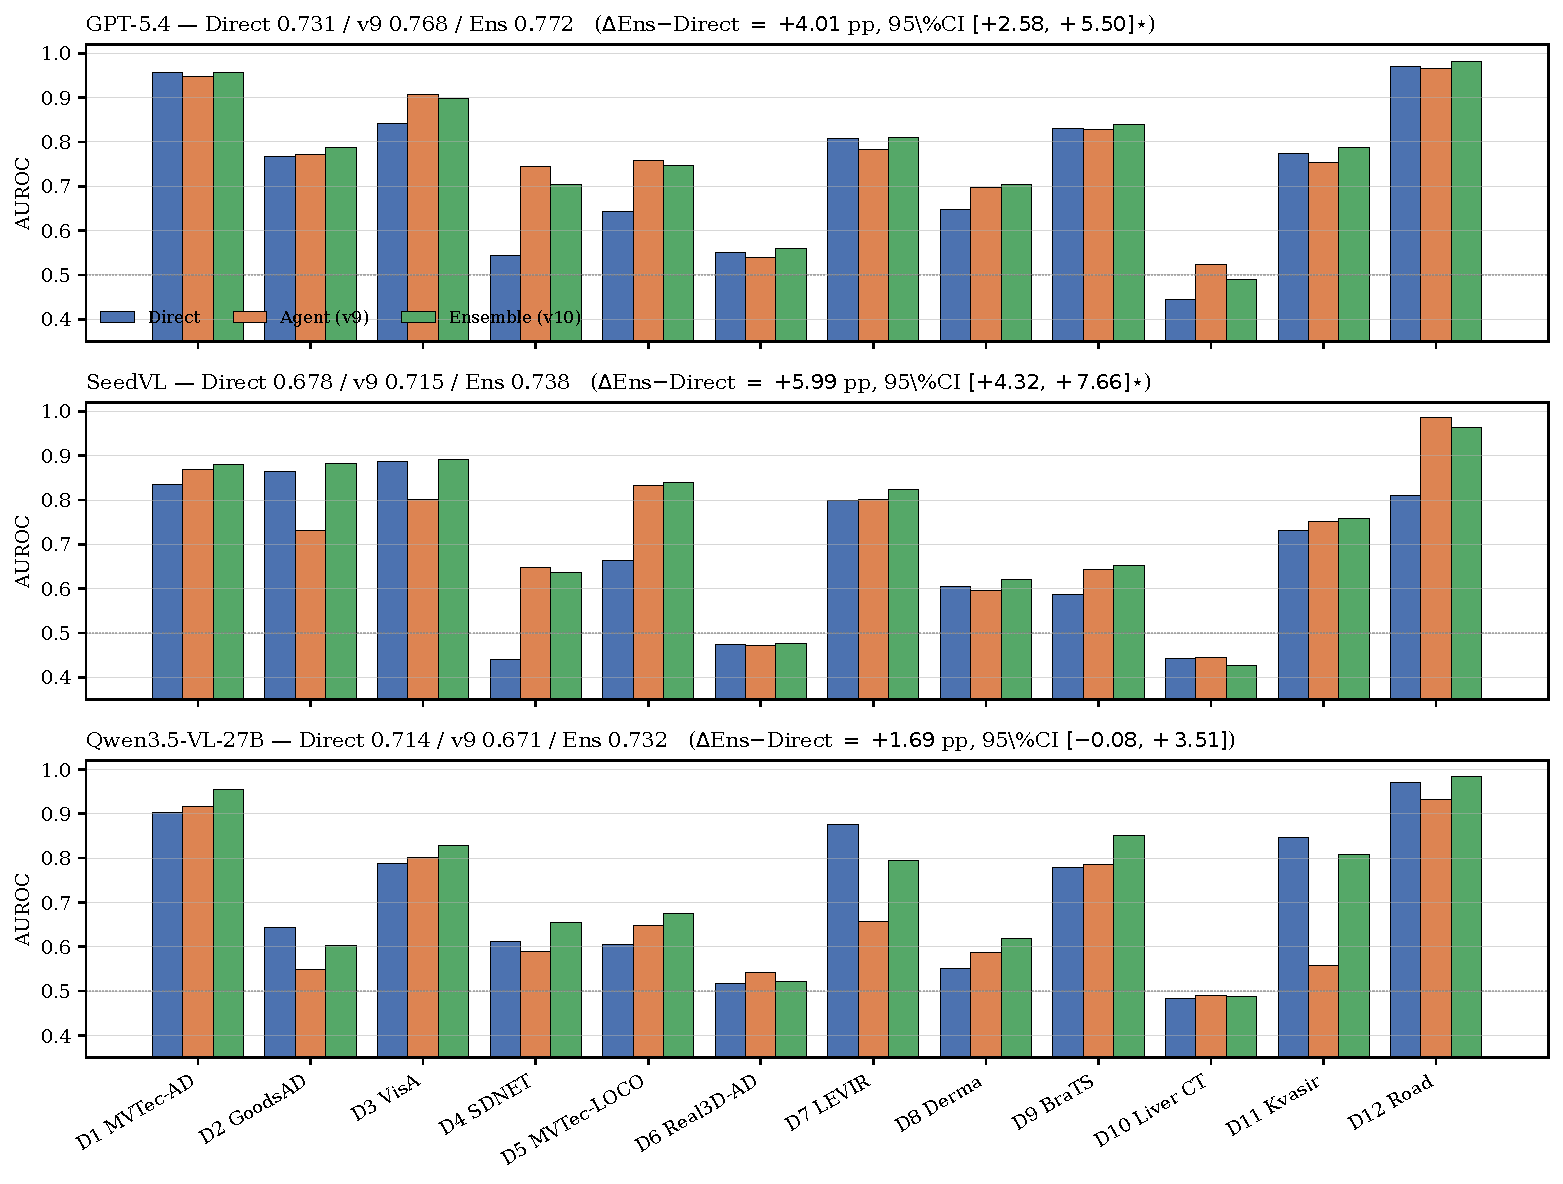
\includegraphics[width=\linewidth]{figures/fig_per_domain.pdf}
\caption{\textbf{Per-domain AUROC on CrossDomainVAD-12 test} ($n{=}1{,}418$), one panel per VLM backbone. Three bars per domain: Direct (blue) / refutation agent alone (orange) / ensemble $0.5\!\cdot\!\text{Direct}+0.5\!\cdot\!\text{the refutation agent}$ (green). Grey dotted line marks the $0.5$ random-guessing floor. Macro numbers and the stratified paired bootstrap $\Delta$(Ens$-$Direct) with $95\%$ CI are reported in each panel title. The ensemble's complementary-error gain concentrates on infrastructure (D4), logical (D5), and road (D12) on SeedVL; on GPT-5.4 the gain is uniform across industrial and medical families; on Qwen3.5-VL-27B the ensemble has to compensate for the refutation agent's deficit on D7 (LEVIR) and D11 (Kvasir) by relying on Direct.}
\label{fig:per_domain_appendix}
\end{figure}

\begin{table}[h]
\centering
\caption{Per-backbone macro AUROC on CrossDomainVAD-12 test ($n{=}1{,}418$, 12 domains, $\ge 90$ valid items per domain after error filtering):  the ensemble's Direct branch, the refutation agent alone, and the ensemble. Headline numbers match Table~\ref{tab:main_results}; full per-domain breakdown in Figure~\ref{fig:per_domain_appendix}. All comparisons use the $1{,}000$-resample stratified paired bootstrap with per-domain stratification.}
\label{tab:per_domain}
\small
\begin{tabular}{lccccccc}
\toprule
Backbone & Direct & the refutation agent & Ens & $\Delta_\text{Ens$-$D}$ & 95\% CI & $P(\Delta{>}0)$ & sig. \\
\midrule
GPT-5.4 & 0.731 & 0.768 & \textbf{0.772} & $+4.01$ & $[+2.58, +5.50]$ & $1.000$ & \checkmark \\
SeedVL  & 0.678 & 0.715 & \textbf{0.738} & $+5.99$ & $[+4.32, +7.66]$ & $1.000$ & \checkmark \\
Qwen3.5 & 0.714 & 0.671 & \textbf{0.732} & $+1.69$ & $[-0.08, +3.51]$ & $0.971$ & (0) \\
\bottomrule
\end{tabular}
\end{table}

\section{Per-domain the specialty-aware variant vs  the ensemble deltas}
\label{app:perdomain_v12}

Table~\ref{tab:perdomain_v12_delta} lists per-domain AUROC for the  the ensemble
baseline and the the specialty-aware variant specialty-aware ensemble (\S\ref{ssec:finding6}) on
the two backbones for which the the specialty-aware variant run completed cleanly ($1418/1418$
items, $0$ errors). Both methods use the same parallel-Direct $+$ the refutation agent
ensemble at $\alpha{=}0.5$; only the tool catalog and agent prompt
differ. $\blacktriangle$ marks domains where the specialty-aware variant improves by $\geq 1$~pp;
$\blacktriangledown$ marks regressions of $\geq 1$~pp.

\begin{table}[h]
\centering
\caption{Per-domain specialty-aware minus baseline AUROC delta for the two backbones whose specialty-aware run completed ($n{=}1418$, $0$ errors each). The macro and bootstrap-CI row matches Table~\ref{tab:v12_vs_v10}. GPT-5.4 is omitted here; its specialty-aware run was blocked by sub2api upstream failure on $D5$--$D12$ and only $345$ valid items remain ($76\%$ API-error rate).}
\label{tab:perdomain_v12_delta}
\small
\setlength{\tabcolsep}{4pt}
\begin{tabular}{ll|ccc|ccc}
\toprule
& & \multicolumn{3}{c|}{\textbf{SeedVL}} & \multicolumn{3}{c}{\textbf{Qwen3.5-VL-27B}} \\
Dom & Dataset &  the ensemble & the specialty-aware variant & $\Delta$~pp &  the ensemble & the specialty-aware variant & $\Delta$~pp \\
\midrule
D1  & MVTec-AD     & 0.880 & 0.891 & $+1.08\blacktriangle$  & 0.955 & 0.956 & $+0.12$ \\
D2  & GoodsAD      & 0.883 & 0.878 & $-0.53$               & 0.603 & 0.649 & $+4.56\blacktriangle$ \\
D3  & VisA         & 0.891 & 0.932 & $+4.06\blacktriangle$  & 0.829 & 0.772 & $-5.60\blacktriangledown$ \\
D4  & SDNET        & 0.637 & 0.706 & $+6.91\blacktriangle$  & 0.654 & 0.672 & $+1.76\blacktriangle$ \\
D5  & MVTec-LOCO   & 0.839 & 0.819 & $-2.00\blacktriangledown$ & 0.674 & 0.673 & $-0.07$ \\
D6  & Real3D-AD    & 0.476 & 0.536 & $+5.99\blacktriangle$  & 0.522 & 0.517 & $-0.53$ \\
D7  & LEVIR        & 0.823 & 0.799 & $-2.41\blacktriangledown$ & 0.794 & 0.842 & $+4.79\blacktriangle$ \\
D8  & Derma        & 0.621 & 0.673 & $+5.15\blacktriangle$  & 0.619 & 0.630 & $+1.09\blacktriangle$ \\
D9  & BraTS        & 0.653 & 0.685 & $+3.24\blacktriangle$  & 0.852 & 0.841 & $-1.07\blacktriangledown$ \\
D10 & Liver CT     & 0.426 & 0.560 & $\mathbf{+13.41\blacktriangle}$ & 0.487 & 0.616 & $\mathbf{+12.91\blacktriangle}$ \\
D11 & Kvasir       & 0.759 & 0.759 & $+0.00$               & 0.809 & 0.817 & $+0.84$ \\
D12 & Road         & 0.963 & 0.969 & $+0.65$               & 0.984 & 0.990 & $+0.68$ \\
\midrule
\multicolumn{2}{l|}{\textbf{Macro}} & \textbf{0.738} & \textbf{0.767} & $\mathbf{+2.90}$ & \textbf{0.732} & \textbf{0.748} & $\mathbf{+2.04}$ \\
\multicolumn{2}{l|}{$95\%$ CI, $P(\Delta{>}0)$}
                                    & \multicolumn{3}{c|}{$[+1.01, +4.85]$, $1.000$}
                                    & \multicolumn{3}{c}{$[+0.05, +4.00]$, $0.981$} \\
\bottomrule
\end{tabular}
\end{table}

The largest per-domain the specialty-aware variant gains are on Liver CT ($+13.4$~pp SeedVL, $+12.9$~pp Qwen3.5) and SDNET concrete ($+6.9$ SeedVL, $+1.8$ Qwen3.5)---both are domains where the new \texttt{tool\_expert\_score} either has strong native signal (D10 subspacead AUROC $0.89$) or where \texttt{tool\_texture\_fft} can detect crack-induced periodicity disruption. Regressions cluster on two failure modes: (a) expert-unavailable industrial domains where the tool ladder over-engages on items  the ensemble correctly resolved at turn~1 (D3 Qwen3.5 $-5.6$~pp); (b) balanced domains where  the ensemble was already near-saturated and the extra variance from the specialty-aware variant's added tool options is net-negative (D5 SeedVL $-2.0$~pp, D7 SeedVL $-2.4$~pp). Nothing in the specialty-aware variant uses dev information, so we do not tune against these regressions; the macro CI on both backbones excludes zero despite the per-domain dispersion.

\section{Leave-one-domain-out sensitivity (full table)}
\label{app:loo}

\begin{table}[h]
\centering
\caption{Leave-one-domain-out macro AUROC gain of score fusion over . All 11 LOO splits are positive on every backbone.}
\label{tab:loo}
\small
\begin{tabular}{lccc}
\toprule
Metric (pp) & GPT-5.4 & SeedVL & Qwen3.5 \\
\midrule
Full $\Delta$ (all 11 domains) & $+$1.4 & $+$1.9 & $+$5.9 \\
LOO min                        & $+$0.9 & $+$1.3 & $+$4.9 \\
LOO max                        & $+$2.2 & $+$3.1 & $+$7.0 \\
LOO std                        & 0.33   & 0.45   & 0.55   \\
Positive splits / 11           & 11 / 11 & 11 / 11 & 11 / 11 \\
\bottomrule
\end{tabular}
\end{table}

\section{Paired bootstrap (full nine-row table) and budget-matched controls}
\label{app:bootstrap}

Table~\ref{tab:bootstrap} in the main body lists the three GPT-5.4 rows; Table~\ref{tab:bootstrap_full} below includes all nine pairwise comparisons across the three backbones. Table~\ref{tab:budget} reports the negative-control budget-matched baselines that we ran on GPT-5.4 and SeedVL calibration splits.

\begin{table}[h]
\centering
\caption{Full stratified paired bootstrap table ($1{,}000$ resamples, per-domain stratification, $n{=}1298$).}
\label{tab:bootstrap_full}
\small
\begin{tabular}{llccc}
\toprule
Backbone & Comparison & $\Delta$ & 95\% CI & sig.\ at $p{<}0.05$ \\
\midrule
\multirow{3}{*}{GPT-5.4}  & fusion vs         & $+0.014$ & $[+0.003, +0.025]$ & \checkmark \\
                           & agent  vs         & $+0.005$ & $[-0.007, +0.015]$ & --- \\
                           & fusion vs agent     & $+0.009$ & $[-0.004, +0.022]$ & --- \\
\midrule
\multirow{3}{*}{SeedVL}   & fusion vs         & $+0.019$ & $[+0.008, +0.031]$ & \checkmark \\
                           & agent  vs         & $+0.023$ & $[+0.007, +0.039]$ & \checkmark \\
                           & fusion vs agent     & $-0.005$ & $[-0.019, +0.010]$ & --- \\
\midrule
\multirow{3}{*}{Qwen3.5}  & fusion vs         & $+0.059$ & $[+0.045, +0.076]$ & \checkmark \\
                           & agent  vs         & $+0.019$ & $[+0.009, +0.030]$ & \checkmark \\
                           & fusion vs agent     & $+0.040$ & $[+0.026, +0.055]$ & \checkmark \\
\bottomrule
\end{tabular}
\end{table}

\begin{table}[h]
\centering
\caption{Budget-matched negative controls (\textbf{/-era numbers, pre-}; included as historical record of disqualified designs and \emph{not comparable} with the ensemble numbers in Table~\ref{tab:main_results}). TheDirect / SubspaceAD fusion / AnomalyClaw rows in this table use our older  descriptor Direct and our  router \texttt{AnomalyClaw} system; the main-paper headline numbers (GPT-5.4 $0.864$, SeedVL $0.809$, Qwen3.5 $0.814$) are from the refutation agent$+$Direct ensemble on the same test split. ``Random escalation'' and ``DINOv2 blend'' are calibration-split numbers for disqualified designs. This table's purpose is only to show that blind second-call escalation and weaker expert blends are negative controls; it should not be read as a competing test-split comparison against our headline  recipe.}
\label{tab:budget}
\small
\begin{tabular}{lcccc}
\toprule
Method & Calls/img & GPT-5.4 & SeedVL & Qwen3.5 \\
\midrule
 Direct                        & 1.00 & 0.822 & 0.795 & 0.792 \\
Random escalation 30\%           & 1.30 & 0.795 & 0.750 & --- \\
 + 0.2$\cdot$DINOv2 blend      & 1.00 & 0.830 & 0.807 & --- \\
\textbf{ + 0.2$\cdot$SubspaceAD fusion} & \textbf{1.00} & \textbf{0.835} & 0.813 & \textbf{0.851} \\
\textbf{AnomalyClaw}             & $\sim$1.3 & 0.826 & \textbf{0.818} & 0.811 \\
\bottomrule
\end{tabular}
\end{table}

\section{VLM$\times$Expert complementarity matrix (full figure)}
\label{app:complementarity}

\begin{figure}[h]
\centering
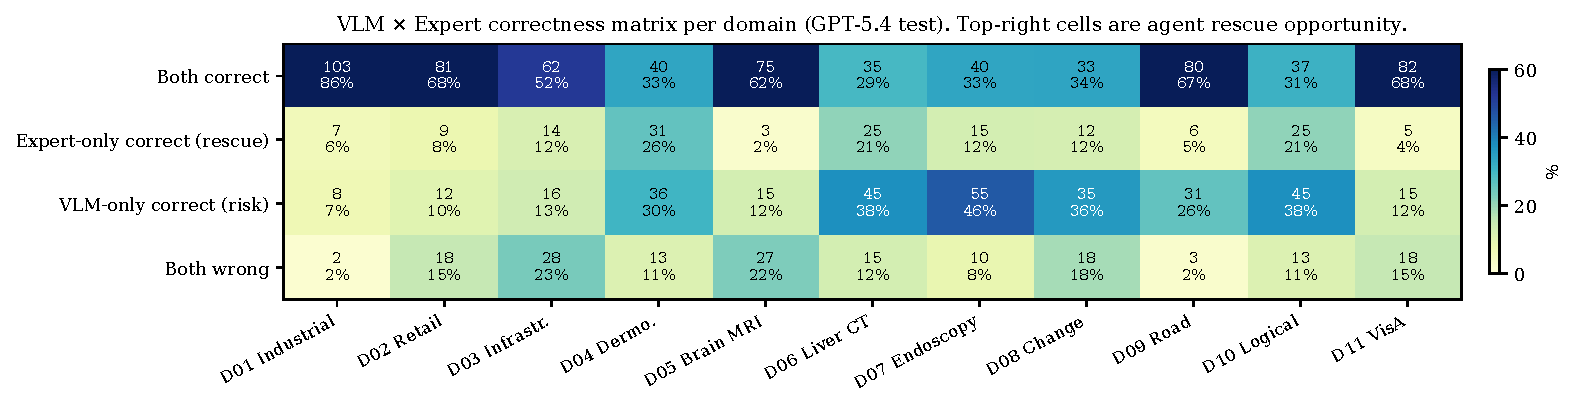
\includegraphics[width=\linewidth]{figures/fig_complementarity.pdf}
\caption{VLM$\times$Expert correctness matrix per domain (GPT-5.4 test). Numbers are \% of items. ``Expert-only correct'' is the upper bound of what the agent can recover; ``VLM-only correct'' is what it risks losing by blindly trusting the expert.}
\label{fig:complementarity}
\end{figure}

\section{AnomalyClaw decision trace example}
\label{app:trace}

Every AnomalyClaw prediction carries a full trace that a human reviewer can audit. For illustration, we show two trace snippets from the actual test runs (Qwen3.5 backbone) — first the autonomous router plan generated for one domain, then a per-item agent execution.

\paragraph{Autonomous router plan (D5c BMAD-Liver, Qwen3.5).}
\begin{quote}\small
\textbf{Strategy:} interpret. \textbf{Expert:} subspacead. \textbf{Tools:} \{\texttt{domain\_descriptor}, \texttt{hotspot\_cropper}\}.\\[2pt]
\textbf{Reasoning (verbatim from Qwen3.5):} ``\emph{SubspaceAD is the designated expert for liver CT texture anomalies, and the interpret strategy provides a critical safety net to verify subtle focal lesions that the VLM may miss. The hotspot cropper makes the second-call evidence explicit when the expert flags a concentrated abnormality.}''\\[2pt]
\textbf{Cost:} 1 text-only VLM call (671 input / 1013 output tokens) — amortised across all 120 D5c test items.
\end{quote}

\paragraph{Per-item agent execution (D1 Industrial, item \texttt{D1\_0063}, SeedVL).}
\begin{quote}\small
\textbf{Phase 1 (Plan lookup).} Cached plan for D1 = (\texttt{strategy:fusion}, \texttt{expert:subspacead}, tools \{\texttt{domain\_descriptor}, \texttt{hotspot\_cropper}\}).\\[2pt]
\textbf{Phase 2 (Expert).} \texttt{SubspaceAD.score} = 17.95 (global calibration median $m{=}40.0$); \texttt{top-5 patches} at $(22,24), (10,24), (10,22), (33,32), (\ldots)$ in the $48{\times}48$ grid. Derived $\rho = 159.7$, $\kappa = 1.43$.\\[2pt]
\textbf{Phase 3 (Online override).} $\hat{y}_{\mathrm{}}{=}$normal AND $\rho > 0.8$ $\Rightarrow$ promote strategy \emph{fusion} $\to$ \emph{interpret}.\\[2pt]
\textbf{Interpret call.} VLM re-examines the cropped hotspot bounding box (image coords $(307, 137)$--$(459, 478)$). \texttt{image\_label}=``anomalous'', \texttt{confidence}=$0.85$, \texttt{evidence}=``a linear scratch visible at the flagged region was missed at global inspection.''\\[2pt]
\textbf{Final decision.} anomaly; score $=$ 0.85. Ground truth: anomalous. Agent escalated correctly via the online expert override.
\end{quote}

Every test-split item has an analogous trace, serialised as JSON in the released \texttt{plan} and \texttt{raw\_output} fields. Score fusion, by contrast, produces only a scalar.

\section{Route C: Component Enumeration prototype}
\label{app:routec}

We prototyped a fourth route, \emph{Component Enumeration} (Route C), for logical anomalies (D10 MVTec-LOCO) where the anomaly is defined by wrong count or wrong spatial arrangement of components rather than by a texture defect. Route C triggers when $\rho{>}1.2$ and $\kappa{<}1.10$ (strong but \emph{dispersed} expert signal). The action is a second VLM call with a specialised enumerate prompt that asks the model to list components in the query versus the references and report count differences.

On D10 calibration (20 items, 4 reference images per query), Route C reaches 60\% accuracy versus 's 55\%. The gain is modest for two reasons: (i) VLMs struggle to count small similar objects reliably, and (ii) the 20-item calibration split yields noisy threshold estimates. Route C is \emph{not} part of the main-table AnomalyClaw variant reported in Table~\ref{tab:main_results}: the reported numbers use only Routes A/B/D. We include Route C here as a concrete direction for future work and flag it as a prototype rather than a validated component of the agent.

\section{Routing distribution}
\label{app:routing}

\begin{figure}[h]
\centering
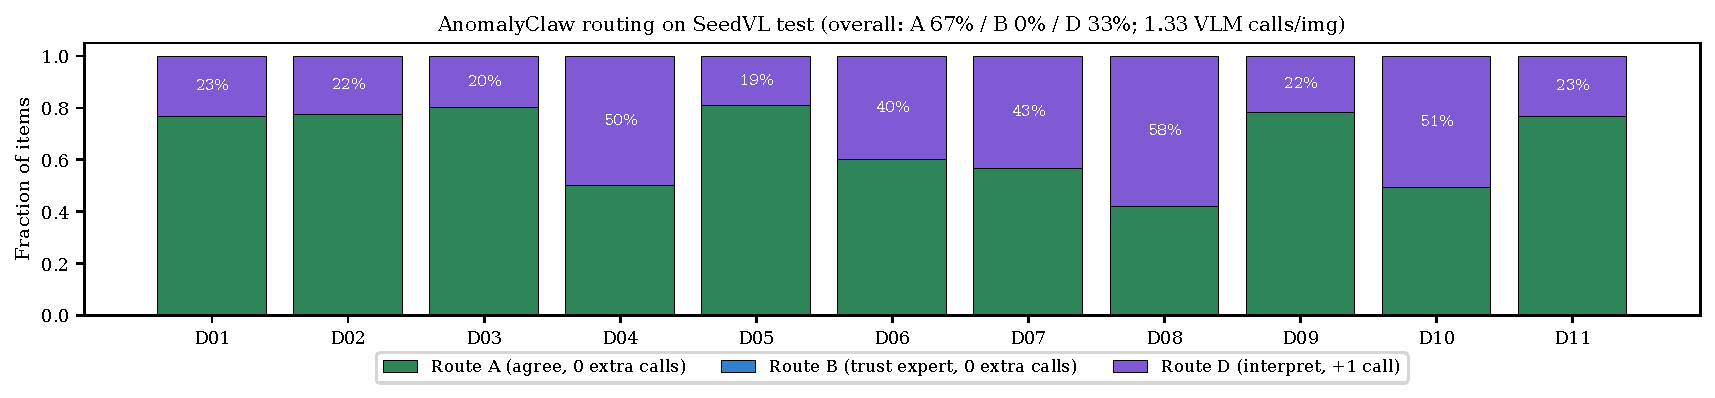
\includegraphics[width=0.75\linewidth]{figures/fig_routing.pdf}
\caption{AnomalyClaw routing distribution on the SeedVL test split. 67\% of items resolve by Route A (VLM and expert agree, 0 extra calls); Route D (interpret) is invoked on 33\% of items; Route B (trust expert) does not fire on any test item because the asymmetric anomaly-trust gate handles strong concentrated signals before they reach Route B.}
\label{fig:routing_appendix}
\end{figure}

\section{Proposer--Advocate debate protocol}
\label{app:debate}

The \emph{debate} strategy runs two VLM calls in sequence. The Proposer receives the query, references, and the task-anchored descriptor, and returns a JSON object \texttt{\{image\_label, anomaly\_type, evidence, confidence, bbox\}}. The Advocate receives the Proposer's output verbatim plus an adversarial prompt asking it to refute the Proposer's claim using the same references, and returns a JSON object \texttt{\{refute\_confidence, counter\_evidence\}}. We combine both into a final score via the rule: if \texttt{refute\_confidence}\,$\geq 0.6$, overturn the Proposer; if \texttt{proposer.confidence}\,$\geq 0.6$ and \texttt{refute\_confidence}\,$\leq 0.4$, commit to the Proposer; otherwise take the Proposer's score unchanged. No third VLM call and no oracle. Temperature is 0 for both calls; the same descriptor $\phi_d$ is used.

\section{Descriptor router rules}
\label{app:router_rules}

The descriptor router maps each domain family to a default strategy. Rules were frozen once from the benchmark descriptor before any test query; no calibration AUROC was consulted.

\begin{table}[h]
\centering
\caption{Descriptor router rules.}
\label{tab:router_rules}
\small
\begin{tabular}{llp{7cm}}
\toprule
Family & Strategy & Reasoning \\
\midrule
industrial / retail / industrial\_visa & fusion & texture-dominant few-shot; expert is reliably discriminative, VLM calibrates \\
infrastructure & fusion & concrete cracks flagged by patch expert; descriptor narrows false positives \\
logical (D9 MVTec-LOCO) & fusion & component structure visible to patch expert; VLM rules out semantic look-alikes \\
dermoscopy (D4) & fusion & patch expert catches localised lesions; VLM rules out imaging artefacts \\
medical\_mixed / liver\_ct / brain\_mri & fusion & SubspaceAD complements VLM on non-trivial intensity shifts \\
gi\_endoscopy (D7, D5d) & direct & VLM-strong: mucosa colour/shape semantics beyond generic feature distance \\
remote-sensing change (D6 LEVIR) & direct & change semantics require descriptor-level task anchoring \\
road (D8, D9 RA21+BDD) & direct & semantic obstacle recognition dominates; expert is a distractor \\
\bottomrule
\end{tabular}
\end{table}

\section{Tool contracts}
\label{app:tools}

Each tool has a small Python contract. Below are the full signatures; the implementations (Python/NumPy) are in \texttt{refine-logs/anomaclaw\_v2/registry.py}.

\begin{itemize}
    \item \texttt{domain\_descriptor(domain\_code) $\to$ str}: returns the task-anchored descriptor. Zero cost, no side effect.
    \item \texttt{reference\_retriever(query, refs, k=3) $\to$ list[int]}: cosine similarity of DINOv2-CLS tokens; returns top-$k$ reference indices.
    \item \texttt{hotspot\_cropper(query, patches, k=5, pad=0.15) $\to$ bbox}: takes the top-$k$ expert patches, computes a padded bounding box in image coordinates, returns a crop for the VLM.
    \item \texttt{component\_counter(hotspot\_map, threshold=0.5) $\to$ (n, stats)}: connected-component labelling with skimage; returns component count and per-component area/centroid.
    \item \texttt{knowledge\_lookup(domain\_code) $\to$ list[str]}: returns a fixed, per-domain keyword list (length $\le 6$; written once during benchmark setup).
\end{itemize}

Tools are composed explicitly by each strategy: \emph{direct} uses only the descriptor; \emph{fusion} uses descriptor and expert scores; \emph{interpret} additionally uses the cropper and expert hotspots; \emph{debate} uses the descriptor and optionally the retriever. No tool is invoked outside its strategy's declared contract.

\section{Rulebook Pilot: L1 invariants + L2 oracle corrective rules}
\label{app:rulebook_pilot}

The domain-rule corpus reused by the Controller (\S\ref{sec:controller},
Stage D) was produced by an earlier pilot that we ran on the same
CrossDomainVAD-12 dev/test split. We document it here for reproducibility;
the pilot's standalone results are not part of the main claim but its
artefacts (per-domain JSON rulebooks) are the \texttt{invariant},
\texttt{corrective\_fn}, and \texttt{corrective\_fp} entries that the  the controller extension
rulebook RAG retrieves.

\paragraph{L1 --- Reference-only invariants.}
For each (domain, category) pair, a reflector VLM (Qwen3.5-VL-27B) is shown
$n{=}8$ normal reference images and asked to list visual \emph{invariants}
--- concrete properties verifiable in \emph{every} reference --- restricted
to six types:
\begin{itemize}[topsep=1pt,parsep=0pt,itemsep=1pt]
  \item \texttt{count}: exact number of parts, segments, or discrete items.
  \item \texttt{symmetry}: axes or symmetries preserved across references.
  \item \texttt{spatial\_layout}: global arrangement of components.
  \item \texttt{color\_palette}: colour range observed across refs.
  \item \texttt{texture}: surface or fabric texture properties.
  \item \texttt{structural}: overall shape, topology, or part connectivity.
\end{itemize}
The reflector is forbidden from listing ``hypothesised anomaly modes'' (an
earlier pilot design that collapsed into generic VLM-prior recitation).
Empty lists are allowed when no invariant can be verified across all
references.

\paragraph{L2 --- Oracle cluster rules.}
For each domain, we run Passive the refutation agent on the $40$-item dev split, form a
balanced batch of $K/2$ false negatives (gt$=$1, $s{<}0.5$) plus $K/2$
false positives (gt$=$0, $s{\ge}0.5$) with $K{=}10$, reveal their manifest
labels, and ask a reflector VLM to propose $1$--$3$ \emph{corrective}
rules per side over the whole batch at once. Per-item rules are forbidden
(they over-generate); \texttt{normal\_tolerance} rules must name a specific
visual feature rather than blanket-suppress an anomaly class.

\paragraph{Rule store.}
For each domain we emit one JSON file containing the invariants and
correctives tagged with metadata:
$(\mathrm{type},\ \mathrm{category}\ [\text{or null}],\ \mathrm{text},\ \mathrm{source\_items},\ \mathrm{confidence})$.
The Controller never consumes these rules directly; instead it reads
RAG-retrieved top-$k$ subsets filtered by the query's $(\mathrm{domain},
\mathrm{category})$ metadata (\S\ref{ssec:ctrl_arch}). The stacked store
size ranges from 10 rules (D12 road safety, single category with few
invariants) to 86 rules (D1 MVTec-AD, eight categories each contributing
count/colour/texture/structural invariants).

\paragraph{Artefacts.}
Per-domain JSON: \texttt{benchmark/results/verbalized/\_l1/} and
\texttt{\_l2/}. The  the controller extension stacked rulebook: \texttt{benchmark/results/verbalized/\_rulebook/}.
